\documentclass[11pt]{standalone}
\usepackage{amssymb}
\usepackage{amsmath}
\usepackage[no-math]{fontspec}
\usepackage{unicode-math}
\usepackage{libertinus}
\usepackage{pgf,xcolor}
\usepackage{tikz}
\usetikzlibrary{arrows.meta, backgrounds, decorations.pathmorphing, patterns}
\usepackage{pgfplots}
\pgfplotsset{compat=newest}

\definecolor{my_darkgray}{HTML}{484949}
\definecolor{my_lightgray}{HTML}{F3F4F4}
\definecolor{my_darkblue}{HTML}{005A94}
\definecolor{my_lightblue}{HTML}{CCDEE9}
\definecolor{my_yellow}{HTML}{FFEC7F}
\definecolor{my_red}{HTML}{E60000}
\definecolor{my_orange}{HTML}{E87846}

\begin{document}
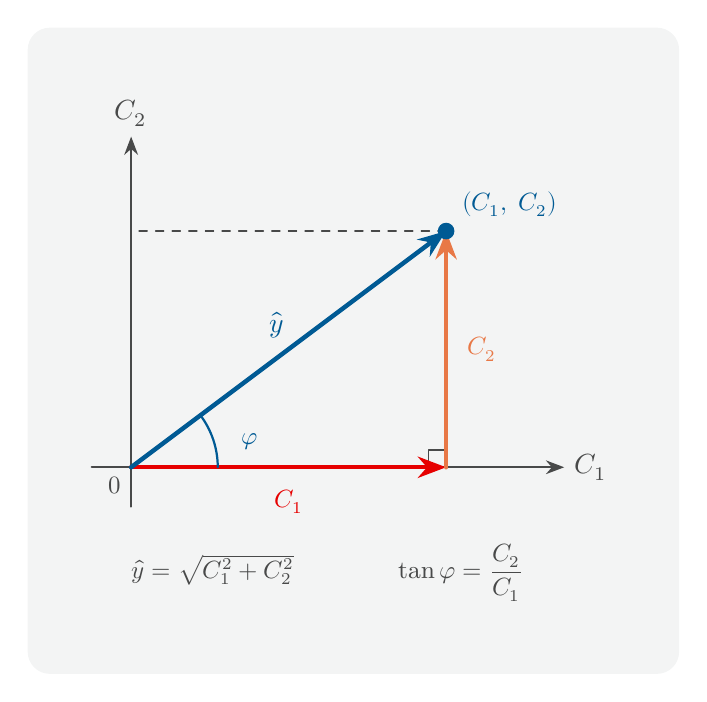
\begin{tikzpicture}[
    show background rectangle,
    background rectangle/.style={fill=my_lightgray, rounded corners=8pt},
    inner frame sep=0.8cm,
    >=Stealth,
    line cap=round,
    line join=round
]

% ======= KOORDINATENACHSEN =======
\draw[->, thick, my_darkgray] (-0.5, 0) -- (5.5, 0)
    node[right, my_darkgray] {$C_1$};
\draw[->, thick, my_darkgray] (0, -0.5) -- (0, 4.2)
    node[above, my_darkgray] {$C_2$};
\node[below left, my_darkgray, font=\small] at (0, 0) {$0$};

% ======= GESTRICHELTE PROJEKTIONSLINIEN =======
% Vertikale Linie vom Punkt zur C₁-Achse
\draw[dashed, thin, my_darkgray] (4, 3) -- (4, 0);
% Horizontale Linie vom Punkt zur C₂-Achse
\draw[dashed, thin, my_darkgray] (4, 3) -- (0, 3);

% ======= RECHTER WINKEL bei (4, 0) =======
\draw[thin, my_darkgray] (3.78, 0) -- (3.78, 0.22) -- (4, 0.22);

% ======= KOMPONENTENPFEILE =======
% Horizontale Komponente C₁ (rot): von O nach (4, 0)
\draw[->, ultra thick, my_red] (0, 0) -- (4, 0);
\node[below, my_red, font=\small] at (2.0, -0.16) {$C_1$};

% Vertikale Komponente C₂ (orange): von (4, 0) nach (4, 3)
\draw[->, ultra thick, my_orange] (4, 0) -- (4, 3);
\node[right, my_orange, font=\small] at (4.15, 1.5) {$C_2$};

% ======= AMPLITUDENVEKTOR ŷ (dunkelblau) =======
% Winkel: arctan(3/4) ≈ 36.87°; Betrag: sqrt(4²+3²) = 5
\draw[->, ultra thick, my_darkblue] (0, 0) -- (4, 3);
\node[above left, my_darkblue] at (2.05, 1.52) {$\hat{y}$};

% ======= WINKELKENNZEICHNUNG φ =======
\draw[thick, my_darkblue]
    (1.1, 0) arc[start angle=0, end angle=36.87, radius=1.1];
\node[my_darkblue, font=\small] at (1.50, 0.33) {$\varphi$};

% ======= PUNKT (C₁, C₂) =======
\fill[my_darkblue] (4, 3) circle (3pt);
\node[above right, my_darkblue, font=\small] at (4.08, 3.06)
    {$(C_1,\;C_2)$};

% ======= FORMELN =======
\node[my_darkgray, font=\small, anchor=north] at (2.5, -0.85)
    {$\hat{y} = \sqrt{C_1^2 + C_2^2}
     \qquad\qquad
     \tan\varphi = \dfrac{C_2}{C_1}$};

\end{tikzpicture}
\end{document}
